%TODO: Find a better way to compare the approaches

\begin{frame}{Learning based}
	\only<1> {
		Most occluded paths over a terrain tend to follow similar trajectories.  \\
		Idea: Compute highly occluded paths between pairs of points and make a sparse network of the common sub-paths
	}
	\only<2> {
		The algorithm for the creating the learning based network follows three stages:
		\begin{enumerate}
			\item Compute optimal paths between pair of points
			\item Identify the sub-paths used by many paths.
			\item Make a network of these sub-paths
		\end{enumerate}
	}
\end{frame}

\begin{frame}{Learning based}{Stage 1}
	\only<1> {
		Pick $n$ points on the bord and for each of these points compute the optimal path to $m$ other points on the border. \\
		This way we get $nm$ paths. 
	}
	\only<2> {
		\centering
		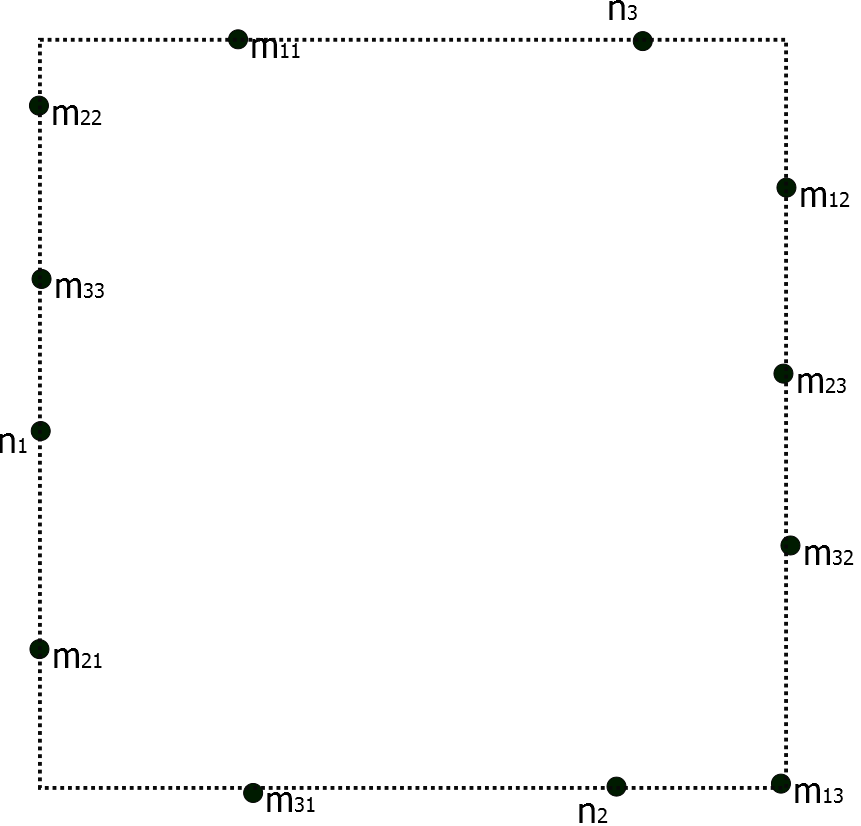
\includegraphics[width=0.6\textwidth]{net-leba1.png}
	}
	\only<3> {
		\centering
		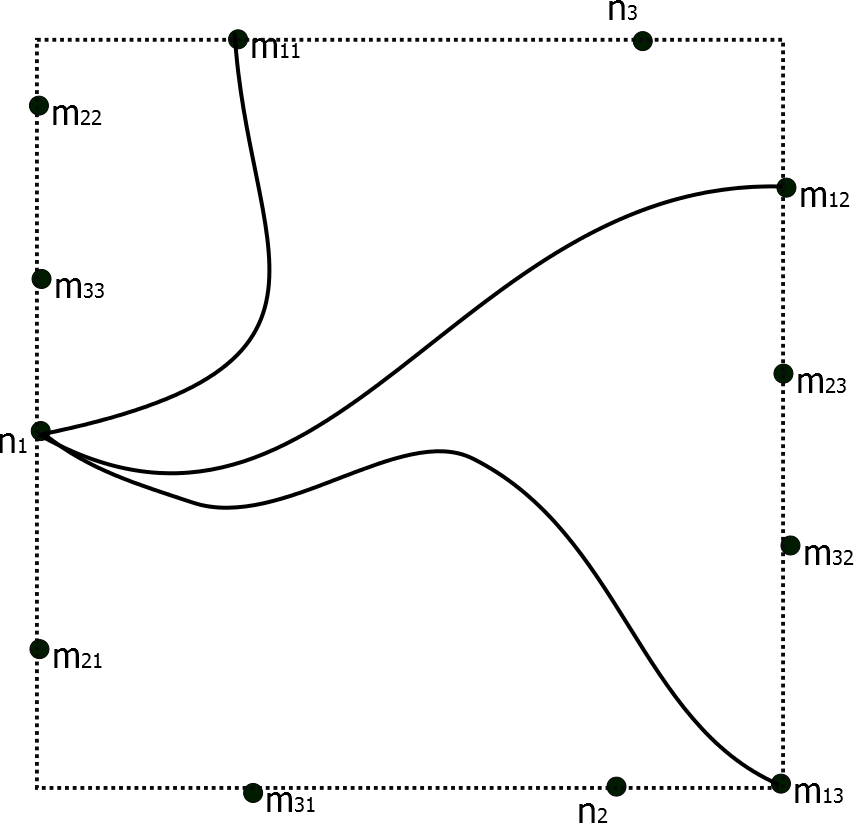
\includegraphics[width=0.6\textwidth]{net-leba2.png}
	}
	\only<4> {
		\centering
		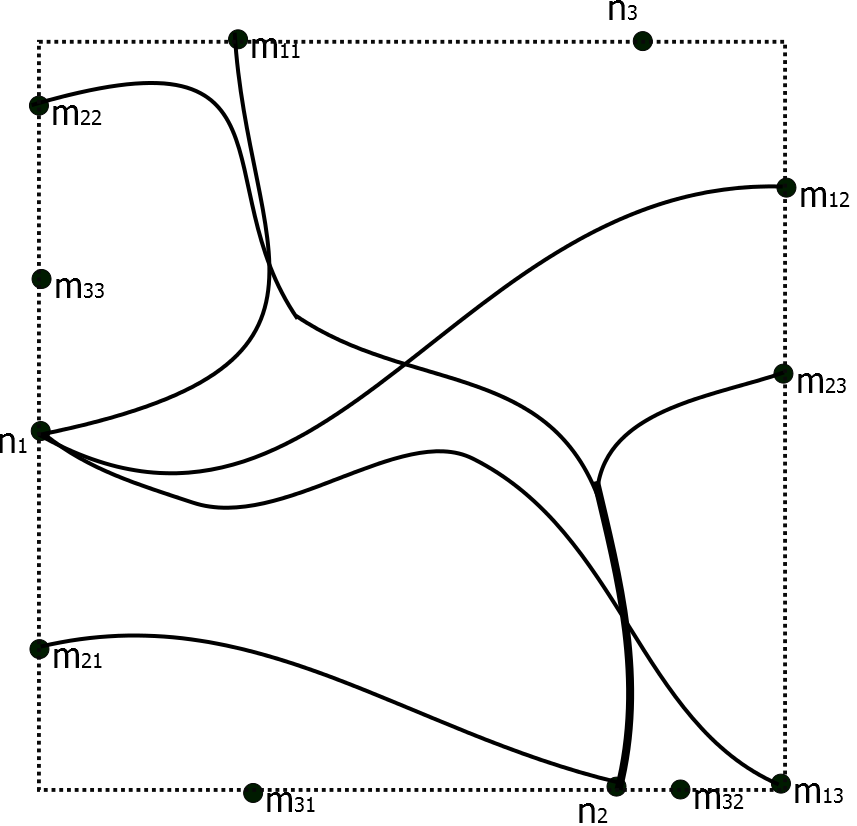
\includegraphics[width=0.6\textwidth]{net-leba3.png}
	}
	\only<5> {
		\centering
		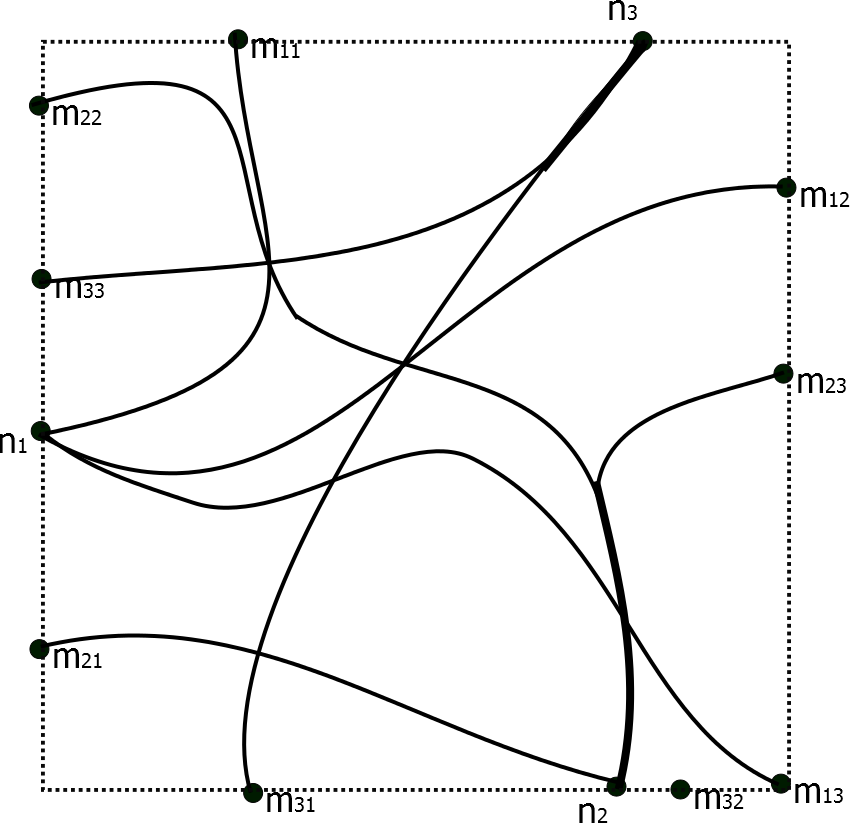
\includegraphics[width=0.6\textwidth]{net-leba4.png}
	}
\end{frame}

\begin{frame}{Learning based}{Stage 2}
	\only<1> {
		Find points for which the number of paths passing through extends a threshold. 
	}
	\only<2> {
		Threshold = 3

		\centering
		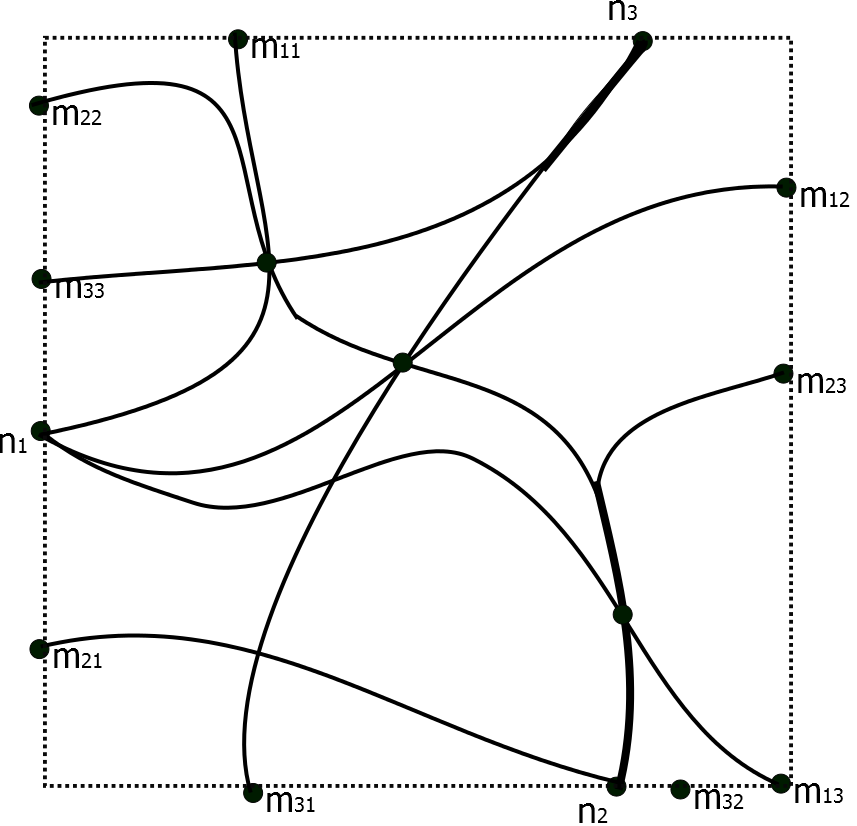
\includegraphics[width=0.5\textwidth]{net-leba5a.png}
	}
	\only<3> {
		Threshold = 3

		\centering
		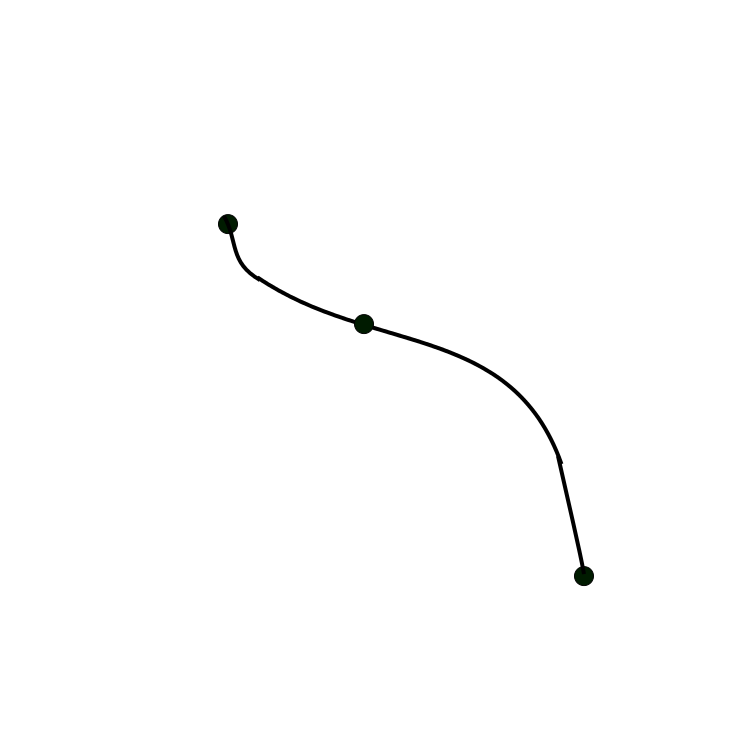
\includegraphics[width=0.5\textwidth]{net-leba6a.png}
	}
	\only<4> {
		Threshold = 2

		\centering
		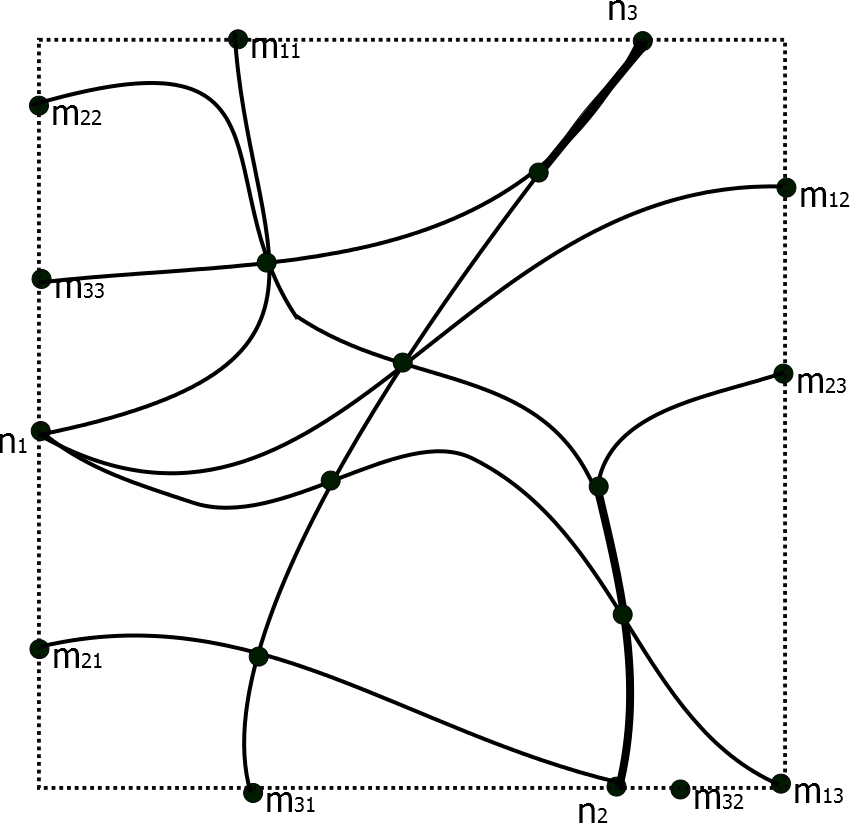
\includegraphics[width=0.5\textwidth]{net-leba5b.png}
	}
	\only<5> {
		Threshold = 2

		\centering
		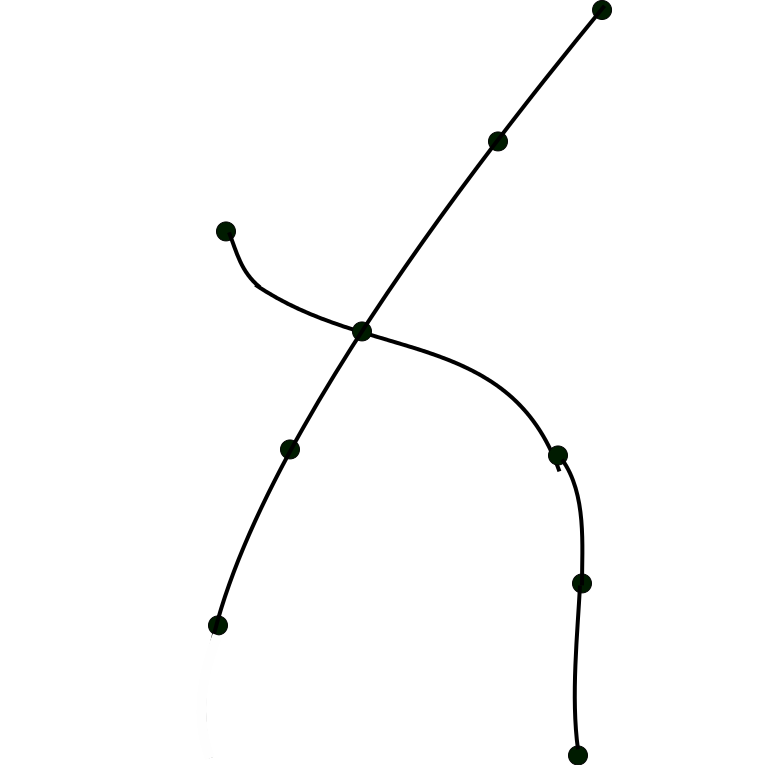
\includegraphics[width=0.5\textwidth]{net-leba6b.png}
	}
\end{frame} 

\begin{frame}{Learning based}{Stage 3}
	\only<1> {
		Make the network complete.
	}

	\only<2> {
		\centering
		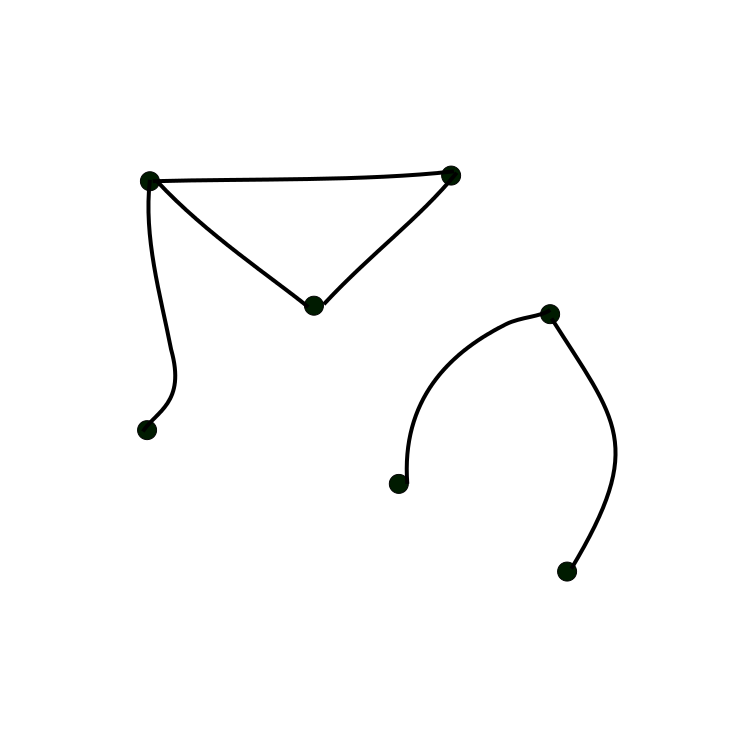
\includegraphics[width=0.6\textwidth]{net-leba7.png}
	}

	\only<3> {
		\centering
		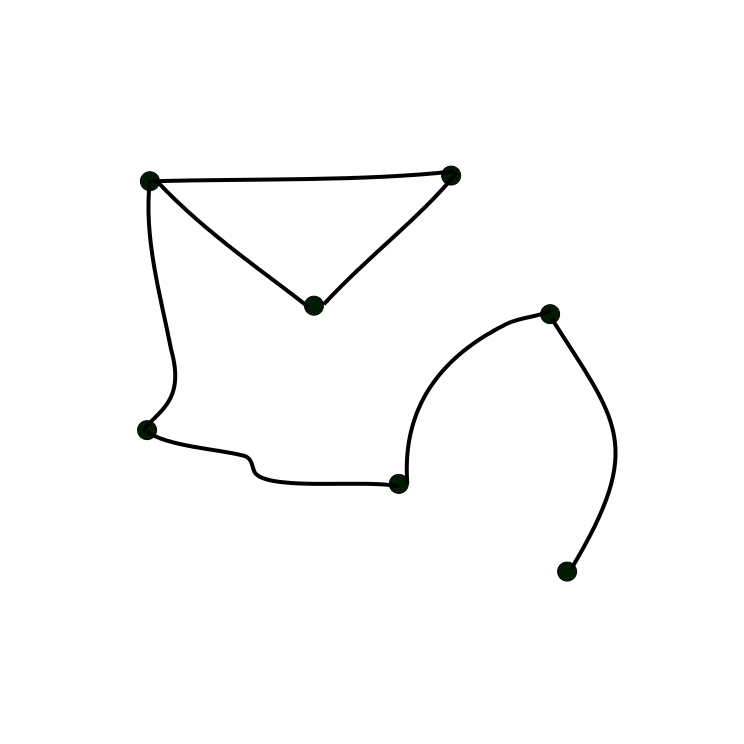
\includegraphics[width=0.6\textwidth]{net-leba8.png}
	}
\end{frame} 

\begin{frame}{Sampling based}

\end{frame}

\begin{frame}{Sampling based}{Result}
	\centering
	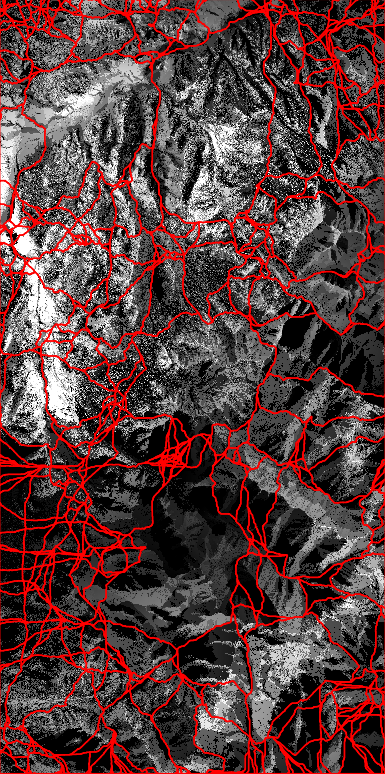
\includegraphics[height=\textwidth,angle=90]{networks-strategies-sampling}
\end{frame}

\begin{frame}{Topology based}

\end{frame}

\begin{frame}{Topology based}{Result}
	\centering
	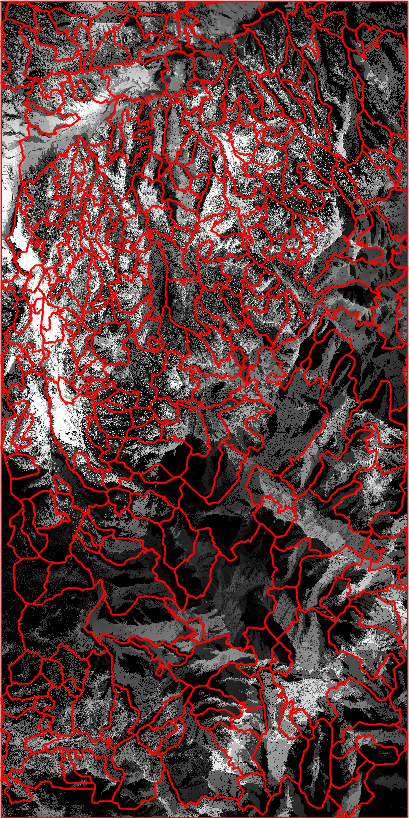
\includegraphics[height=\textwidth,angle=90]{networks-strategies-topology}
\end{frame}

